
\section{USB Gadget / OTG Mode ZeroConf (Raspberry Pi Zero)}


Beim USB-Gadget oder OTG-Betrieb kann die Raspberry Pi Zero direkt �ber den Micro-USB-Anschluss mit einem PC oder Laptop verbunden werden. Er verh�lt sich dann wie ein USB-Ger�t und kann z.~B. ein Massenspeicher-, Serielles-  oder Netzwerkger�t simulieren.\\
Verh�lt er sich als Netzwerkger�t kann eine Netzwerkverbindung �ber ein virtuelles Netzwerk zum Ger�t hergestellt werden. 
Weitere Informationen �ber den OTG-Betrieb kann der Git-Hub Seite  \url{https://gist.github.com/gbaman/50b6cca61dd1c3f88f41} entnommen werden.

\subsection{Client - Raspberry Pi Zero}

Nach der Einrichtung des Betriebssystems auf der MicroSD-Karte m�ssen noch ein paar Modifikationen an den Dateien der Boot-Partition durchgef�hrt werden. 

Folgender Text muss nach der Anweisung "`rootwait"' in die Datei "`cmdline.txt"' eingef�gt werden:
\begin{screensmall}
modules-load=dwc2,g_ether g_ether.host_addr=00:01:02:03:04:05 g_ether.dev_addr=00:01:02:03:04:06
\end{screensmall}

Die Angabe der MAC-Adresse f�r Host und Ger�t ist optional, es wird aber empfohlen da sonst diese Adressen zuf�llig vergeben werden. Die Werte k�nnen frei gew�hlt werden, sollten sich aber nicht mit den Adressen im Netz bzw. Host �berschneiden.\\

Folgende Zeile muss am Ende in die Datei "`config.txt"' hinzugef�gt werden:
\begin{screensmall} 
dtoverlay=dwc2
\end{screensmall}

Weiters muss eine leere Datei mit dem Namen "`ssh"' erzeugt werden, damit der SSH-Dienst automatisch nach dem Start ausgef�hrt wird. Danach kann die MicroSD-Karte in den Raspberry Pi Zero gesteckt und �ber ein MicroUSB-Kabel an einen Computer angeschlossen werden. 
Es ist zu beachten, dass das MicroUSB-Kabel am mittleren MicroUSB-Anschluss angeschlossen werden muss!\\

%\begin{console} 
%	touch /mnt/ssh
%\end{console} 

%Wird Microsoft Windows verwendet so muss das Programm Bonjour von Apple installiert werden. 
%Falls der Dienst noch nicht von einem Apple Programm (iTunes oder Quicktime) installiert wurde, kann von der Seite \url{https://support.apple.com/kb/DL999?locale=de_AT} ein Setup heruntergeladen werden.\\

\subsection{Host - Kubuntu 16.04 (Zeroconf)}

Die Konfiguration der IP-Adressen erfolgt �ber das Zero Configuration Networking System (Zeroconf). Dazu muss am Host-PC der Dienst Avahi (avahi-daemon) installiert sein. Dieser ist auf den meisten Linux Systemen bereits vorinstalliert.\\ 
  
Zur Konfiguration unter Linux Kubuntu 16.04 muss zuerst "`Netzwerkverbindungen"' ge�ffnet werden. 
Dazu klickt man mit der rechten Maustaste auf das Netzwerksymbol in Infobereich rechts unten. Nun kann die Option "`Netzwerkverbindungen einrichten..."' ausgew�hlt werden.

\begin{figure}[ht]
  \centering
  
\includegraphics[scale=1.0]{images/OTG_NetzwerkverbindungenIcon.png}	
  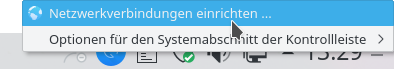
\includegraphics[scale=0.42]{images/OTG_NetzwerkverbindungenOpen.png}	
  %	\caption{}
  \label{OTG_LINUX_NetzwerkverbindungenApp}
\end{figure}


Danach kann die neue "`Kabelnetzwerkverbindung"' umbenannt werden, z.~B. in Raspberry Pi Zero. Erkennen kann man das Netzwerk an der Mac-Adresse die man bei "`g\_ether.host\_addr"' angegeben hat (z.~B. 00:01:02:03:04:05).  


\begin{figure}[ht]
  \centering
  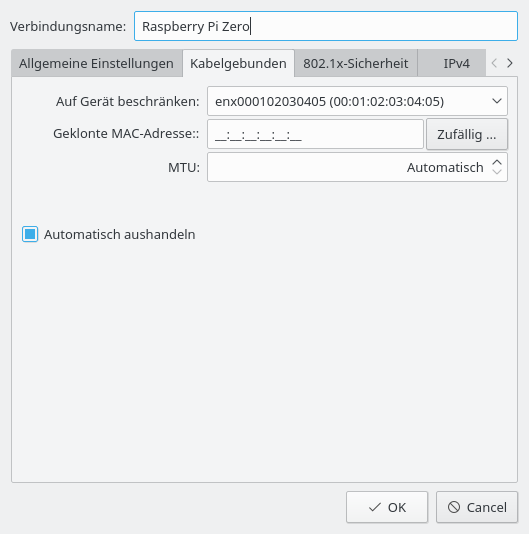
\includegraphics[scale=0.45]{images/OTG_Pi_Verbindungsname.png}
	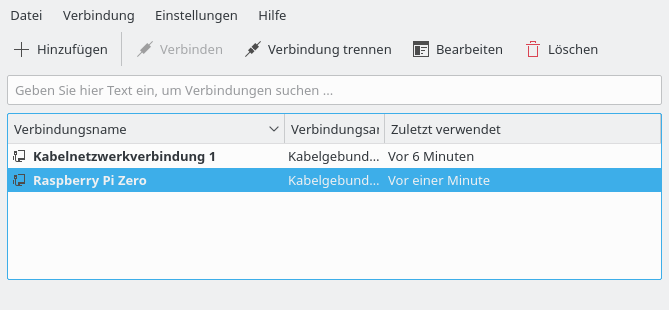
\includegraphics[scale=0.45]{images/OTG_Netzwerkverbindungen.png}
%	\caption{}
  \label{OTG_LINUX_Netzwerkverbindungen}
\end{figure}


Am Host-PC muss bei den IPv4-Einstellungen Methode "`Link-Local"' eingestellt sein.  


\begin{figure}[ht]
  \centering
  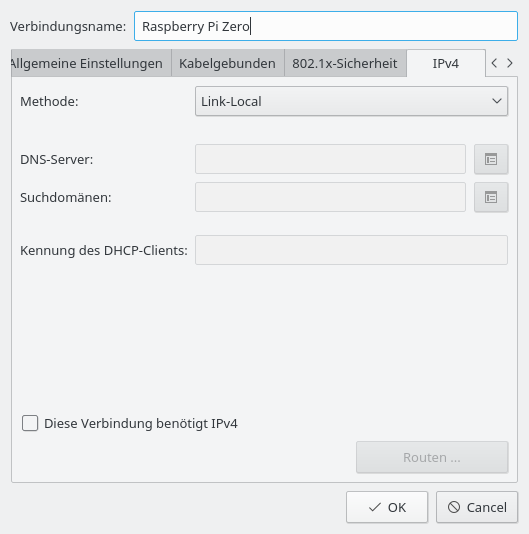
\includegraphics[scale=0.45]{images/OTG_IPv4.png}
%	\caption{}
  \label{OTG_LINUX_IPV4}
\end{figure}


%\subsection{Internet Zugriff} 
~\\
Nach der Einrichtung des Netzwerk kann der Raspberry Pi Zero mit dem Namen "`raspberrypi.local"' erreicht werden. Um den Raspbery Pi Zero mit dem Internet verbinden zu k�nnen m�ssen einige Einstellungen am Host %und Client
 gemacht werden. Man muss den Name des Netzwerkger�ts am Host-PC kennen, das mit dem Internet verbunden ist. Dies ermittelt man �ber die Netzwerkeinstellungen oder �ber die Konsole mit nmcli. Im Beispielfall ist der Name "`enp0s25"' das richtige Ger�t.

\begin{console} 
	nmcli d
\end{console} 

\begin{screensmall} 
	GER�T            TYP       STATUS           VERBINDUNG        
	enx000102030405  ethernet  verbunden        Raspberry Pi Zero 
	enp0s25          ethernet  verbunden        Netzwerkverbindung 1                
	lo               loopback  nicht verwaltet  --  
\end{screensmall}

Damit der Internetzugang f�r den Raspberry Pi Zero freigegeben wird, m�ssen am Host-PC folgende Befehle in einem Terminal eingeben werden. "`enp0s25"' muss durch den Namen des Netzwerkger�ts ersetzt werden, das mit dem Internet verbunden ist.

\begin{console} 
	sudo sysctl -w net.ipv4.ip_forward=1
	sudo iptables -t nat -A POSTROUTING -o enp0s25 -j MASQUERADE
\end{console}



Sp�ter wird noch die IP-Adresse der lokalen Raspberry Pi Verbindung ben�tigt. Dies ermittelt man in der Konsole mit dem Befehl \texttt{ifconfig}.  

\begin{console} 
	ifconfig enx000102030405 | head -n 2
\end{console}

\begin{screensmall} 
	enx000102030405 Link encap:Ethernet  Hardware Adresse 00:01:02:03:04:05  
	inet Adresse:169.254.144.15  Bcast:169.254.255.255  Maske:255.255.0.0
\end{screensmall}





Nach der Einrichtung kann per SSH-Client eine Verbindungen zum Raspberry Pi hergestellt werden. Dazu muss in einem Terminal folgender Befehl eingegeben werden:

\begin{console} 
	ssh -X pi@raspberrypi.local
\end{console}

Um grafische Programme am Host anzeigen zu k�nnen, muss der Parameter \texttt{-X} angegeben werden. "`\textbf{pi}"' ist der Standardbenutzer am System. Dann wird eine X-Server Verbindung via SSH hergestellt. Verbindet man sich zum ersten Mal mit dem Raspberry Pi, so wird noch eine Sicherheitswarnung ausgegeben. Der kryptographische Schl�ssel f�r die Verbindung ist dem lokalen System noch nicht bekannt.%  und muss best�tigt werden.
\begin{screensmall}
The authenticity of host 'raspberrypi.local (192.168.137.10)' can't be established.
ECDSA key fingerprint is SHA256:Dcf3HYgE2GHnNnZ8Xhv8iJ9yA+zvfXBC9COm2eL9i0w.
Are you sure you want to continue connecting (yes/no)? 
Warning: Permanently added 'raspberrypi.local,192.168.137.10' (ECDSA) to the list of known hosts.
\end{screensmall}

Die Frage muss mit \texttt{yes} best�tigt werden. Anschlie�end muss das Default-Passwort von Raspbian "`\textbf{raspberry}"' eingegeben werden. Nun sollte man den Raspberry Pi Prompt \texttt{pi@rasbperrypi:\textasciitilde  \$} sehen. 

Wechselt man zu einem anderen Raspberry Pi mit den gleichen Namen oder installiert das System nochmals, so kann es passieren, dass eine Fehlermeldung ausgegeben wird, weil sich der kryptographische Schl�ssel ge�ndert hat.

\begin{screensmall} 
@@@@@@@@@@@@@@@@@@@@@@@@@@@@@@@@@@@@@@@@@@@@@@@@@@@@@@@@@@@
@    WARNING: REMOTE HOST IDENTIFICATION HAS CHANGED!     @
@@@@@@@@@@@@@@@@@@@@@@@@@@@@@@@@@@@@@@@@@@@@@@@@@@@@@@@@@@@
\end{screensmall} 

%The ECDSA host key for raspberrypi.local has changed,
%and the key for the corresponding IP address 169.254.229.192
%is unknown. This could either mean that
%DNS SPOOFING is happening or the IP address for the host
%and its host key have changed at the same time.
%@@@@@@@@@@@@@@@@@@@@@@@@@@@@@@@@@@@@@@@@@@@@@@@@@@@@@@@@@@@
%@    WARNING: REMOTE HOST IDENTIFICATION HAS CHANGED!     @
%@@@@@@@@@@@@@@@@@@@@@@@@@@@@@@@@@@@@@@@@@@@@@@@@@@@@@@@@@@@
%IT IS POSSIBLE THAT SOMEONE IS DOING SOMETHING NASTY!
%Someone could be eavesdropping on you right now (man-in-the-middle attack)!
%It is also possible that a host key has just been changed.
%The fingerprint for the ECDSA key sent by the remote host is
%SHA256:Dcf2HYyE2GHnNpZ8Xhv8iJ9yj+zvfXBC9COm2eL9i0w.
%Please contact your system administrator.
%Add correct host key in /home/evil/.ssh/known_hosts to get rid of this message.
%Offending ECDSA key in /home/evil/.ssh/known_hosts:9
%remove with:
%ssh-keygen -f "/home/evil/.ssh/known_hosts" -R raspberrypi.local
%ECDSA host key for raspberrypi.local has changed and you have requested strict checking.

In diesem Fall muss man die Verbindung aus den bekannten Hosts l�schen. Hierf�r muss folgendes Kommando ausgef�hrt werden:

\begin{console} 
	ssh-keygen -R raspberrypi.local
\end{console}

Optional kann auch der Parameter \texttt{-o UserKnownHostsFile=/dev/null} beim ssh-Befehl hinzugef�gt werden. Dann erfolgt keine �berpr�fung der Verbindung. 

~\\
Nun muss noch der Gateway am Client eingestellt werden. Dazu muss die IP-Adresse des Host-PC bekannt sein. Im Beispiel muss die IP-Adresse "`169.254.144.15"' durch die IP-Adresse des Hosts ersetzt werden.   


\begin{console} 
	sudo route add default gw 169.254.144.15
\end{console}

\clearpage
\section{USB Gadget / OTG Mode DHCP-Server (Raspberry Pi Zero)}

\begin{figure}[ht]
	\centering
	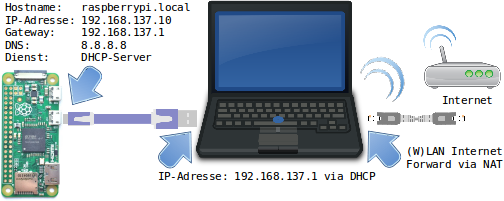
\includegraphics[scale=0.9]{images/Aufbau_Schema.png}
	%	\label{Aufbau_Schema}
\end{figure}

\subsection{Client - Statische IP-Adresse und DHCP Server}

Die folgende Einstellungen m�ssen nicht gemacht werden, erleichtern aber das Arbeiten. Der Raspberry Pi Zero hat dann eine statische IP-Adresse und kann leichter angesprochen und auch die Internetverbindung freigegeben werden (vor allem mit Microsoft Windows 7 und 10).\\
Am Client-System, also der Raspberry Pi Zero, kann die Netzwerkadresse, der Gateway und ein DNS-Server eingestellt werden. Dieser Schritt ist unbedingt n�tig wenn die Internetverbindung unter Windows dem Ger�t zur Verf�gung gestellt werden soll. Die IP-Adresse die eingestellt wird, muss f�r Windows 7 aus dem Bereich 192.168.137.* sein (z.~B. 192.168.137.10). Der Gateway ist die IP-Adresse des Host-PC. Als DNS-Server kann z.~B. der Server von Google mit der Adresse 8.8.8.8 verwendet werden. Die Einstellungen k�nnen in der Konfigurationsdatei f�r den DHCP-Client definiert werden.\\ 
Die IP-Adresse des Host-Computers kann via eines DHCP-Server konfiguriert werden. Das hat den Vorteil, dass dort keine Konfiguration des Netzwerks erfolgen muss. Es wird zur weiteren Einrichtung ein Terminalzugang zum Einplatinencomputer ben�tigt und eine Internetverbindung sollte bestehen damit man den DHCP-Server installieren kann.\\
Per SSH-Client kann eine Verbindungen zum Raspberry Pi mit dem Befehl "'ssh pi@raspberrypi.local"' hergestellt werden. %Nun kann die Konfiguration abgeschlossen werden.   

\begin{console}
	sudo vi /etc/dhcpcd.conf
\end{console}

Folgende Zeilen m�ssen am Ende der Datei eingef�gt werden:\\

\filename{/etc/dhcpcd.conf [-rw-r-{-}r-{-} root root]}
\begin{file}
	
# define static profile for Pi 
profile static_usb0
static ip_address=192.168.137.10/24
static routers=192.168.137.1
static domain_name_servers=8.8.8.8

# static profile on usb0
interface usb0 
fallback static_usb0
\end{file}


\begin{console}
	sudo apt-get update
	sudo apt-get install isc-dhcp-server
\end{console}

%Falls die Internetverbindung am Raspberry Pi Zero nicht m�glich ist, kann der Server auch manuell heruntergeladen, auf der Boot-Partition gespeichert und installiert werden.\\
%Install-Datei:
%\url{http://archive.raspbian.org/raspbian/pool/main/i/isc-dhcp/isc-dhcp-server_4.3.5-3_armhf.deb}
%	
%	\begin{console}
%		sudo dpkg -i /boot/isc-dhcp-server_4.3.1-6+deb8u2_armhf.deb
%	\end{console}
%	
%	Nach der Installation kann der DHCP-Server parametriert werden. 
	
\begin{console}
	sudo vi /etc/dhcp/dhcpd.conf
\end{console}

%ddns-update-style none;

%#option domain-name "example.org";
%#option domain-name-servers ns1.example.org, ns2.example.org;

%default-lease-time 600;
%max-lease-time 7200;
%
%log-facility local7;


Folgende Zeilen m�ssen am Ende der Datei eingef�gt werden:\\

\filename{/etc/dhcp/dhcpd.conf [-rw-r-{-}r-{-} root root]}
\begin{file}
subnet 192.168.137.0 netmask 255.255.255.0{
	range 192.168.137.2 192.168.137.9;
	option broadcast-address 192.168.137.255;
}

#USB OTG Host-PC set IP-Address to 192.168.137.1
host USB_OTG_HOST {
	hardware ethernet 00:01:02:03:04:05;
	fixed-address 192.168.137.1;
}
\end{file}

\begin{console}
	sudo reboot
\end{console}


\subsection{Host (DHCP-Client)}

\subsubsection{Windows 7}

Nach dem Boot wird automatisch ein neues "`RNDIS/Ethernet Gadget"' erkannt und Treiber installiert. Sollte die Installation nicht erfolgreich abgeschlossen werden k�nnen, so muss man den Treiber manuell installieren.

\begin{figure}[ht]
  \centering
  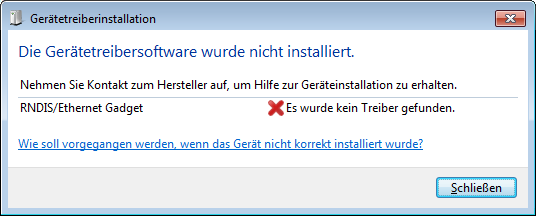
\includegraphics[scale=0.42]{images/OTG_Win7_InstallFail.png}
%  \caption{Windows Treiber konnte nicht automatisch installiert werden}
  \label{OTG_Win7_InstallFail}
\end{figure}

\begin{figure}[ht]
  \centering
  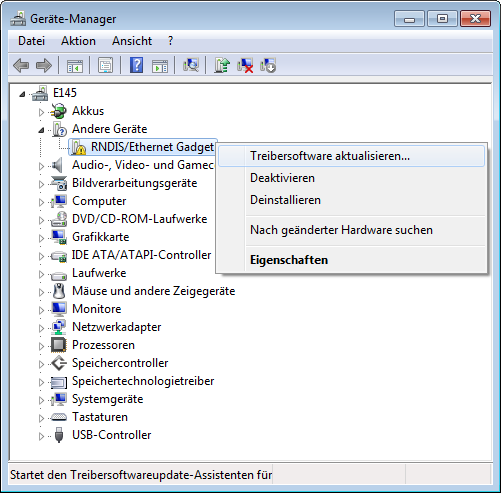
\includegraphics[scale=0.42]{images/Geraetemanager.png}
%  \caption{Windows Treiber konnte nicht automatisch installiert werden}
  \label{OTG_Win7_InstallManual}
\end{figure}

%Dazu �ffnet man den Gr�temanager, aktiviert das fehlerhafte Ger�t unter "`Andere Ger�te"' und �ffnet mit der rechten Maustaste das Kontextmen�. 
Dazu �ffnet man zuerst den Gr�temanager. Dann �ffnet man das Kontextmen� in dem man die rechten Maustatste am 
fehlerhaften Ger�t (Andere Ger�te / RNDIS/Ethernet Gadget) dr�ckt. Nun w�hlt man den Men�punkt "`Treiber Software aktualisieren..."' aus. Im folgenden Dialog w�hlt man "`Auf dem Computer nach Treibersoftware suchen"' und dann "`Aus einer Liste von Ger�tetreibern auf dem Computer ausw�hlen"'. Danach kann der Ger�tetyp gew�hlt werden in dem man "`Netzwerkadapter"' ausw�hlt. Dann w�hlt man den Hersteller "`Microsoft Corporation"' und den Netzwerkadapter "`Remote NDIS based Internet Sharing Device"'. Sollte eine Kompatibilit�tswarnung angezeigt werden, kann der Treiber trotzdem installiert werden. Zum Schluss sollte der Treiber automatisch erfolgreich installiert werden.\\ 

\begin{figure}[ht]
  \centering
  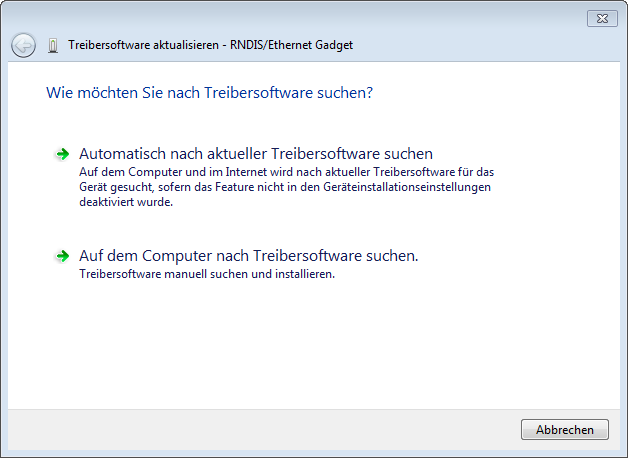
\includegraphics[scale=0.42]{images/OTG_Win7_Install_1.png}
	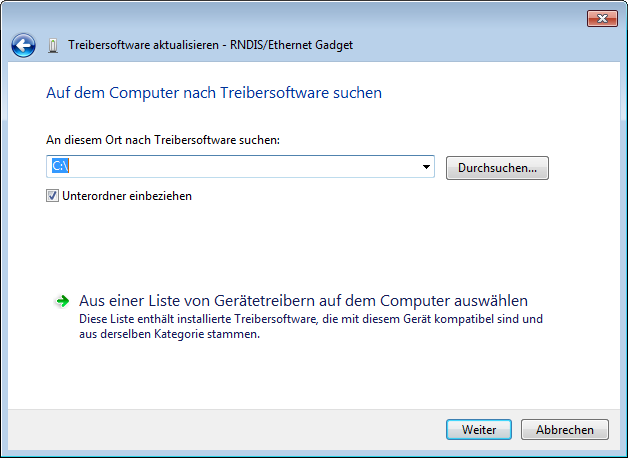
\includegraphics[scale=0.42]{images/OTG_Win7_Install_2.png}
 
%  \caption{}
  \label{OTG_Win7_Install_12}
\end{figure}

\begin{figure}[ht]
  \centering
  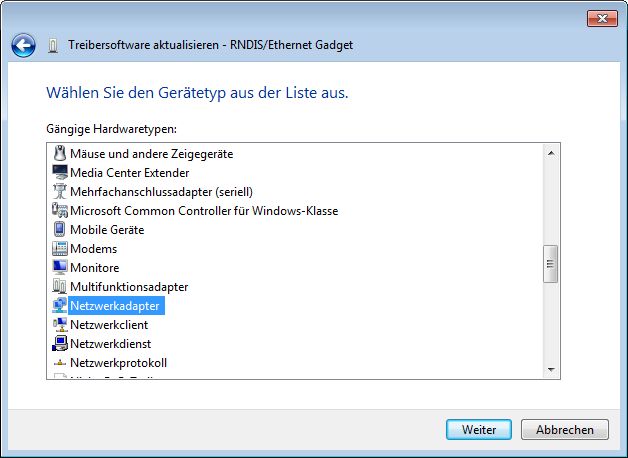
\includegraphics[scale=0.42]{images/OTG_Win7_Install_3.png}
  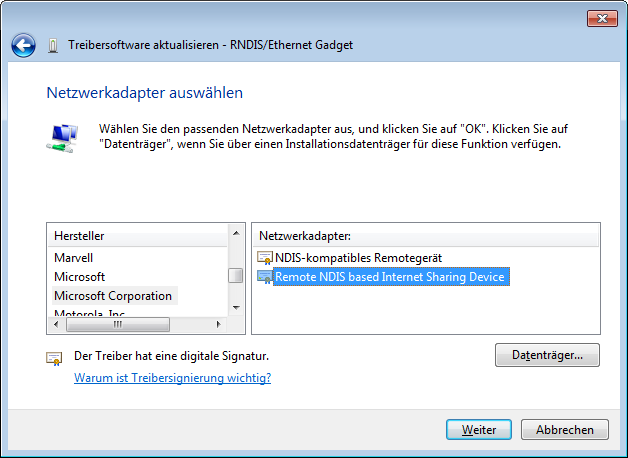
\includegraphics[scale=0.42]{images/OTG_Win7_Install_4.png}
%  \caption{}
  \label{OTG_Win7_Install_34}
\end{figure}


\begin{figure}[ht]
  \centering
  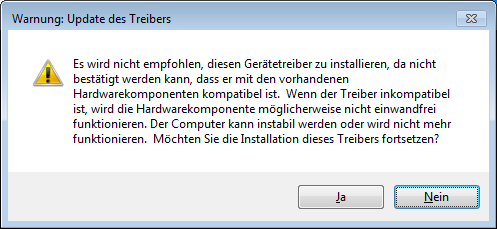
\includegraphics[scale=0.50]{images/OTG_Win7_Install_5.png}
  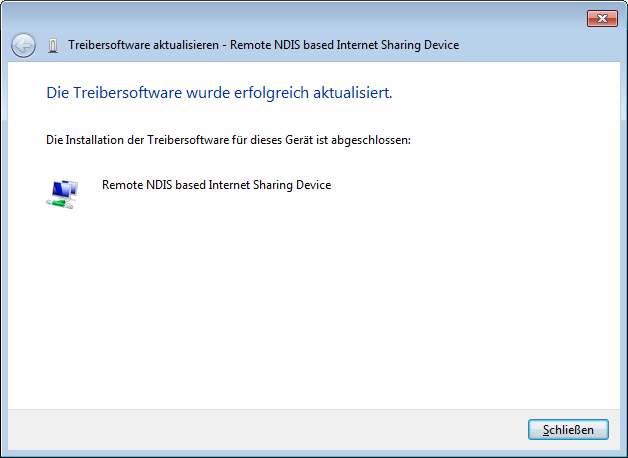
\includegraphics[scale=0.42]{images/OTG_Win7_Install_6.png}
%	\caption{}
  \label{OTG_Win7_Install_56}
\end{figure}


Damit am Ger�t Internet funktionieren kann, muss das Internet f�r das neue Netzwerk freigegeben werden. Dazu �ffnet man das Einstellungs-Fenster f�r die Netzwerkverbindungen. 

\begin{figure}[ht]
  \centering
  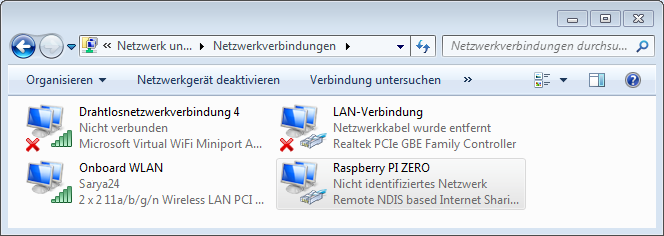
\includegraphics[scale=0.42]{images/OTG_Win7_Netzwerkverbindungen.png}
%	\caption{}
  \label{OTG_Win7_Netzwerkverbindungen}
\end{figure}

Zuerst kann man dem Netzwerkger�t "`Remote NDIS based Internet Sharing Device"' einen neuen Namen geben, z.~B. Raspberry PI ZERO. Nun muss das Netzwerk gesucht werden, das mit dem Internet verbunden ist, z.~B. Onboard WLAN. Bei den Eigenschaften zu dem Netzwerk kann der Reiter "`Freigabe"' ausgew�hlt werden. Danach kann man die Einstellung "`Anderen Benutzern im Netzwerk gestatten, diese Verbindung des Computers als Internetverbindung zu verwenden"' aktivieren und bei Heimnetzwerkverbindung kann das Netzwerk "`Raspberry PI ZERO"' ausgew�hlt werden.\\
Windows 7 legt dann fest, dass die Netzwerkadresse 192.168.137.1 sein muss. Alternativ kann die Verbindung auch zuvor schon auf diese statische IP-Adresse gesetzt werden.\\



\begin{figure}[ht]
  \centering
  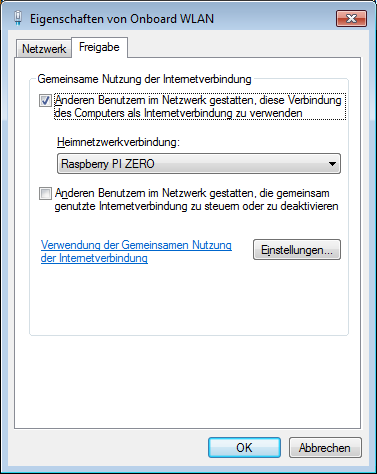
\includegraphics[scale=0.42]{images/OTG_Win7_Inet.png}
  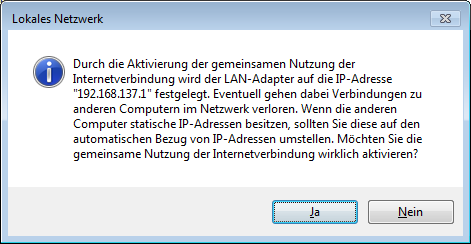
\includegraphics[scale=0.42]{images/OTG_Win7_Inet2.png}
%	\caption{}
  \label{OTG_Win7_Inet_12}
\end{figure}


Nun kann die Verbindung zur Raspberry Pi mit dem Programm Putty und der Adresse "`192.168.137.10"', �ber das SSH-Protokoll hergestellt werden.\\  
Mit dem Befehl "`ping 8.8.8.8"' kann die Internetverbindung getestet werden. Mit dem Befehl "`ping google.com"' kann dann der DNS-Server �berpr�ft werden.   


\clearpage
\subsection{Windows 10}

Nach dem Boot wird der Raspberry Pi Zero als "`Serielles USB-Ger�t"' erkannt und keine korrekten Treiber installiert. Dies muss manuell erfolgen. Dazu l�dt man sich zuerst den zertifizierten Treiber "`Acer Incorporated. - Other hardware - USB Ethernet-RNDIS Gadget"' von der Microsoft Homepage herunter \url{http://download.windowsupdate.com/msdownload/update/driver/drvs/2012/12/20342322_4b9970e3174b23b5cb2371af0837f939a71271ea.cab} bzw. \url{https://tinyurl.com/y6onwaax}. Die ben�tigten Dateien sind in der komprimierten CAB-Datei enthalten. Durch einen Doppelklick auf der Datei kann der Inhalt dargestellt werden. Mit der rechten Maustaste und dem Kontexmen� k�nnen die Dateien z.~B. nach \path{c:\Drivers\RNDIS\} extrahiert werden. 

\begin{figure}[ht]
  \centering
  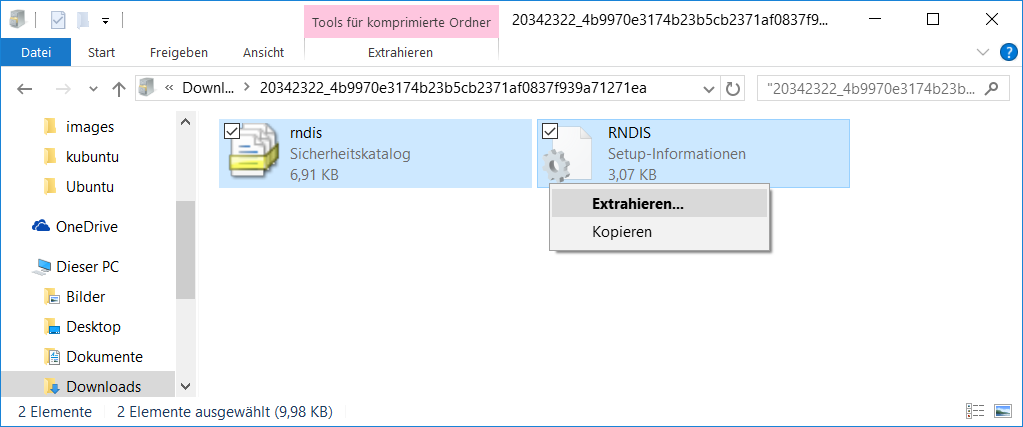
\includegraphics[scale=0.42]{images/OTG_Win10_Install_0.png}
%  \caption{}
  \label{OTG_Win10_Drivers}
\end{figure}

Nun muss der Gr�temanager ge�ffnet werden. Dann �ffnet man das Kontextmen� in dem man die rechte Maustaste am 
"`Serielles USB-Ger�t"' Eintrag dr�ckt. Nun w�hlt man den Men�punkt "`Treiber Software aktualisieren..."' aus. Im folgenden Dialog w�hlt man "`Auf dem Computer nach Treibersoftware suchen"' und dann gibt man das Verzeichnis an, in dem die Treiberdaten extrahiert wurden, z.~B. \path{c:\Drivers\RNDIS\}. Zum Schluss sollte der Treiber automatisch erfolgreich installiert werden.\\ 

\begin{figure}[ht]
  \centering
  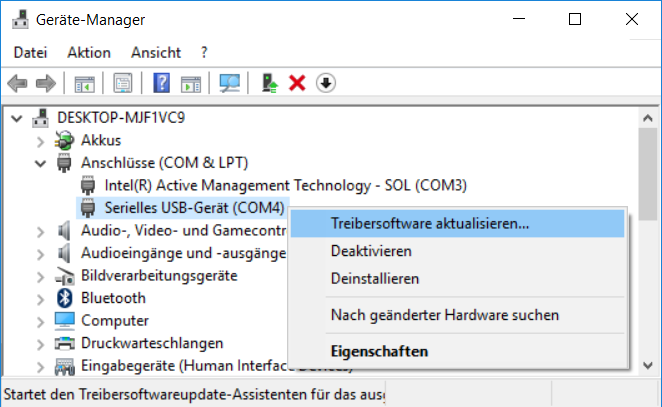
\includegraphics[scale=0.5]{images/OTG_Win10_Install_1.png}
  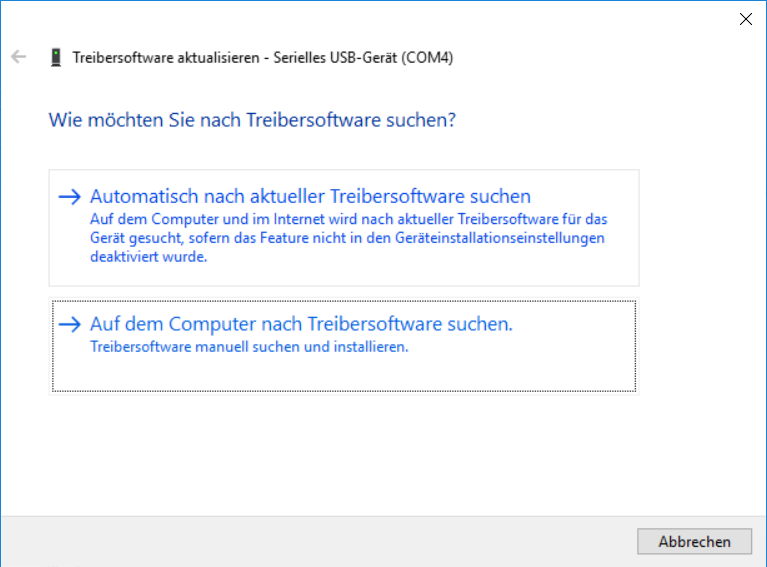
\includegraphics[scale=0.4]{images/OTG_Win10_Install_2.png}
%  \caption{}
  \label{OTG_Win10_Install_1}
\end{figure}


\begin{figure}[ht]
  \centering
  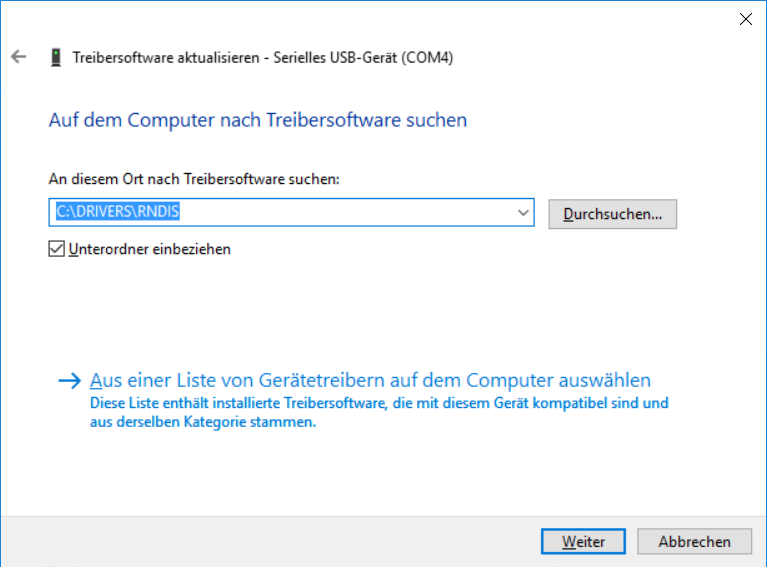
\includegraphics[scale=0.4]{images/OTG_Win10_Install_3.png}
  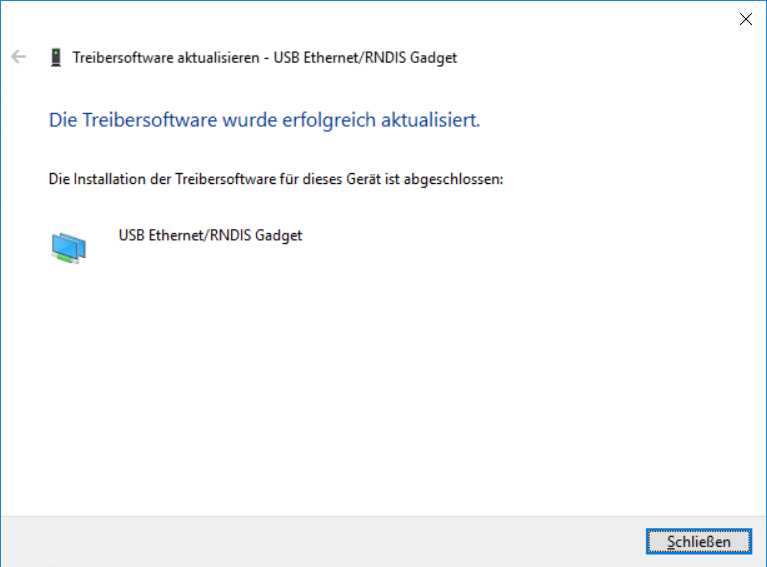
\includegraphics[scale=0.4]{images/OTG_Win10_Install_4.png}
%  \caption{}
  \label{OTG_Win10_Install_3}
\end{figure}  


Damit am Ger�t Internet funktionieren kann, muss das Internet f�r das neue Netzwerk freigegeben werden. Dazu �ffnet man das Einstellungs-Fenster f�r die Netzwerkverbindungen. 

\begin{figure}[ht]
  \centering
  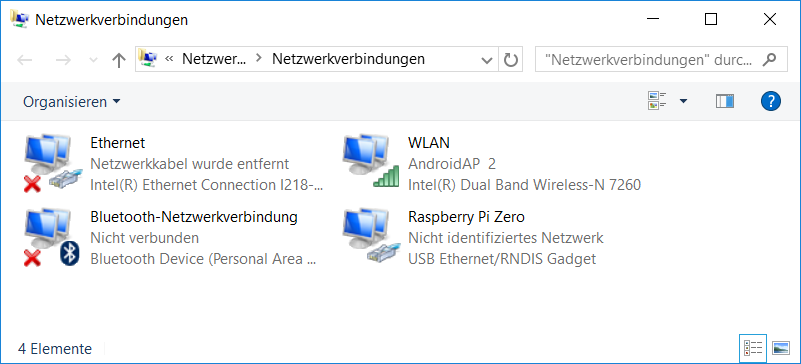
\includegraphics[scale=0.40]{images/OTG_Win10_Netzwerkverbindungen.png}
  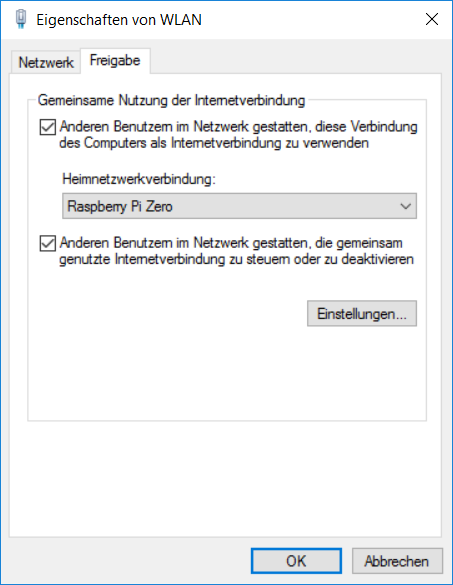
\includegraphics[scale=0.40]{images/OTG_Win10_Inet.png}
%	\caption{}
  \label{OTG_Win10_Netzwerkverbindungen}
\end{figure}

Zuerst kann man dem Netzwerkger�t "`USB Ethernet/RNDIS Gadget"' einen neuen Namen geben, z.~B. Raspberry Pi Zero. Nun muss das Netzwerk gesucht werden, das mit dem Internet verbunden ist, z.~B. WLAN. Bei den Eigenschaften zu dem Netzwerk kann der Reiter "`Freigabe"' ausgew�hlt werden. Danach kann man die Einstellung "`Anderen Benutzern im Netzwerk gestatten, diese Verbindung des Computers als Internetverbindung zu verwenden"' aktivieren und bei Heimnetzwerkverbindung kann das Netzwerk "`Raspberry Pi Zero"' ausgew�hlt werden.\\

Nun kann die Verbindung zur Raspberry Pi mit dem Programm Putty und der Adresse "`raspberrypi.local"', �ber das SSH-Protokoll hergestellt werden (siehe Kapitel \ref{sec:connection_putty} \titleref{sec:connection} - \titleref{sec:connection_putty}).\\  
Mit dem Befehl "`ping 8.8.8.8"' kann die Internetverbindung getestet werden. Mit dem Befehl "`ping google.com"' kann dann der DNS-Server �berpr�ft werden .   

\clearpage
\subsubsection{Kubuntu 16.04}

Am Host-PC muss bei den IPv4-Einstellungen die Methode "`Automatisch"' eingestellt sein. Wenn es sich um eine neue Verbindung handelt, ist dies bereits voreingestellt, eine Parametrierung kann dann entfallen. Ansonsten muss zur Konfiguration unter Linux (Kubuntu 16.04) zuerst der Dialog "`Netzwerkverbindungen"' ge�ffnet werden.\\ 
Dazu klickt man mit der rechten Maustaste auf das Netzwerksymbol in Infobereich rechts unten. Dann kann die Option "`Netzwerkverbindungen einrichten..."' ausgew�hlt werden.

\begin{figure}[ht]
  \centering
  
\includegraphics[scale=1.00]{images/OTG_NetzwerkverbindungenIcon.png}	
  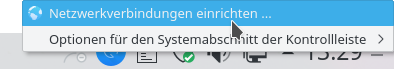
\includegraphics[scale=0.42]{images/OTG_NetzwerkverbindungenOpen.png}	
  %	\caption{}
  \label{OTG_LINUX_NetzwerkverbindungenApp}
\end{figure}


Nun k�nnte die neue "`Kabelnetzwerkverbindung"' umbenannt werden, z.~B. in Raspberry Pi Zero. Erkennen kann man das Netzwerk an der Mac-Adresse, die man bei "`g\_ether.host\_addr"' angegeben hat (z.~B. 00:01:02:03:04:05).  


\begin{figure}[ht]
  \centering
  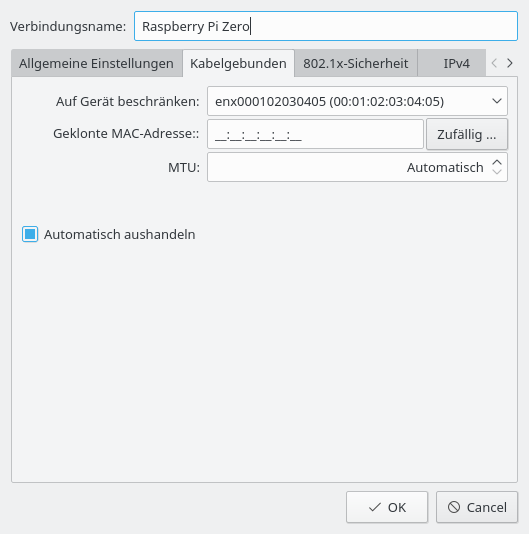
\includegraphics[scale=0.42]{images/OTG_Pi_Verbindungsname.png}
	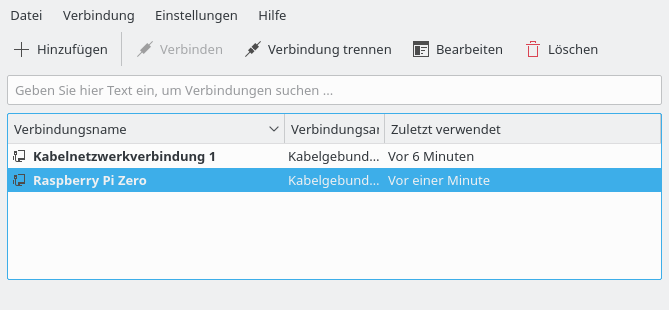
\includegraphics[scale=0.42]{images/OTG_Netzwerkverbindungen.png}
%	\caption{}
  \label{OTG_LINUX_Netzwerkverbindungen}
\end{figure}


Nun kann bei den IPv4-Einstellungen die Methode "`Automatisch"' eingestellt werden.

%\begin{figure}[ht]
%  \centering
%  \includegraphics[scale=0.42]{images/OTG_NetzwerkverbindungenAutomatisch.png}
%	\caption{}
%  \label{OTG_LINUX_Netzwerkverbindungen}
%\end{figure}

\clearpage
%\input{OTG_Mint}



